%%%%%%%%%%%%%%%%%%%%
%
% Parcours noir pour l'activit� TSP
% 
% Author: Marie Pelleau
%
%%%%%%%%%%%%%%%%%%%%

\documentclass{article}

\usepackage{macros}

\titre{noir}{19}

\begin{document}
  \Large
  
  \maketitle
  
  \textbf{Combinatoire : } $\displaystyle{\frac{1}{2} \times (19 - 1)! = 3\,201\,186\,852\,864\,000}$

  \bigskip
    
  \bigskip
  \centering
  
  \begin{tikzpicture}
    \node[inner sep = 0pt] () at (0,0) {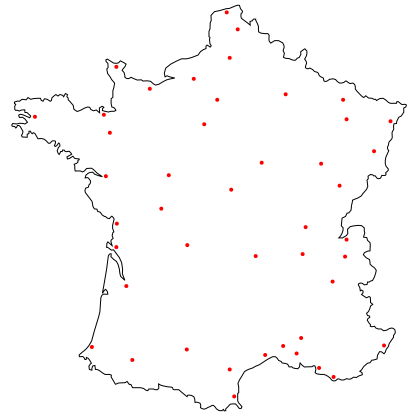
\includegraphics[scale = 1.5]{../france.pdf}};
    
    \node[ville, vvert] (amiens) at (1.005491386, 6.342726704) {}; 
    \node[ville, vvert] (arles) at (3.841548395, -6.186719186) {}; 
    \node[ville, vvert] (carcassonne) at (1.005491386, -6.863986532) {}; 
    \node[ville, vvert] (limoges) at (-0.7935, -1.594) {}; 
    \node[ville, vvert] (macon) at (4.2225, -0.832) {}; 
    \node[ville, vvert] (nancy) at (5.95800885, 3.739480345) {}; 
    \node[ville, vvert] (nice) at (7.54535419, -5.848085513) {}; 
    \node[ville, vvert] (pau) at (-3.1216065, -6.461859045) {}; 
    \node[ville, vvert] (rennes) at (-4.074013704, 3.168036022) {}; 
    
    \node[ville, vbleu] (bourges) at (1.0689852, 0.755271104) {}; 
    \node[ville, vbleu] (clermont) at (2.106050823, -2.0596213) {}; 
    
    \node[ville, vrouge] (avignon) at (4.032029836, -5.530616445) {}; 
    \node[ville, vrouge] (montpellier) at (2.508178309, -6.250213) {}; 
    \node[ville, vrouge] (nimes) at (3.270104072, -5.869250118) {}; 
    
    \node[ville, vnoir] (caen) at (-2.380845341, 5.030521222) {}; 
    \node[ville, vnoir] (chambery) at (5.894515036, -2.080785905) {}; 
    \node[ville, vnoir] (chartres) at (-0.073903445, 3.5278343) {};  
    \node[ville, vnoir] (cherbourg) at (-3.798873845, 5.961763822) {}; 
    \node[ville, vnoir] (poitiers) at (-1.894059436, -0.048983868) {}; 
    
    
    \node[ville] (annecy) at (5.95800885, -1.36118935) {};
    \node[ville] (auxerre) at (2.360026077, 1.89815975) {};
    \node[ville] (besan�on) at (5.661704386, 0.924587941) {};
    \node[ville] (biarritz) at (-4.835939468, -5.911579327) {};
    \node[ville] (bordeaux) at (-3.375581754, -3.329497573) {};
    \node[ville] (brest) at (-7.248704386, 3.845303368) {};
    \node[ville] (calais) at (0.878503759, 8.268705718) {};
    \node[ville] (colmar) at (7.1220621, 2.384945654) {};
    \node[ville] (dijon) at (4.878614018, 1.855830541) {};
    \node[ville] (grenoble) at (5.365399922, -3.139016132) {};
    \node[ville] (laRochelle) at (-3.777709241, -0.683922005) {};
    \node[ville] (lille) at (1.344125059, 7.549109163) {};
    \node[ville] (lyon) at (4.09552365, -1.974962882) {};
    \node[ville] (marseille) at (4.709297181, -6.800492718) {};
    \node[ville] (metz) at (5.809856618, 4.564899922) {};
    \node[ville] (nantes) at (-4.243330541, 1.326715427) {};
    \node[ville] (paris) at (0.476376273, 4.564899922) {};
    \node[ville] (perpignan) at (1.195972827, -8.006875177) {};
    \node[ville] (reims) at (3.375927095, 4.797710572) {};
    \node[ville] (rouen) at (-0.518360141, 5.453813313) {};
    \node[ville] (royan) at (-3.798873845, -1.678658418) {};
    \node[ville] (saintMalo) at (-4.327988959, 3.929961786) {};
    \node[ville] (strasbourg) at (7.820494049, 3.654821927) {};
    \node[ville] (toulon) at (5.407729131, -7.1814556) {};
    \node[ville] (toulouse) at (-0.814664605, -6.01740235) {};
    \node[ville] (tours) at (-1.576590368, 1.369044636) {};
  \end{tikzpicture}
  
  \begin{tikzpicture}
    \draw [white] (0, 10) -- (4, 11); 
    
    \node[inner sep = 0pt] () at (0,0) {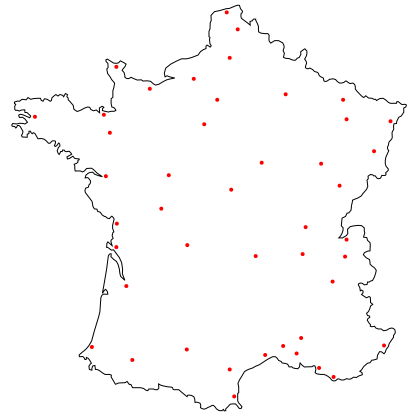
\includegraphics[scale = 1.5]{../france.pdf}};
    
    \node[ville, vnoir] (amiens) at (1.005491386, 6.342726704) {}; 
    \node[ville, vnoir] (arles) at (3.841548395, -6.186719186) {}; 
    \node[ville, vnoir] (carcassonne) at (1.005491386, -6.863986532) {}; 
    \node[ville, vnoir] (limoges) at (-0.7935, -1.594) {}; 
    \node[ville, vnoir] (macon) at (4.2225, -0.832) {}; 
    \node[ville, vnoir] (nancy) at (5.95800885, 3.739480345) {}; 
    \node[ville, vnoir] (nice) at (7.54535419, -5.848085513) {}; 
    \node[ville, vnoir] (pau) at (-3.1216065, -6.461859045) {}; 
    \node[ville, vnoir] (rennes) at (-4.074013704, 3.168036022) {}; 
    
    \node[ville, vnoir] (bourges) at (1.0689852, 0.755271104) {}; 
    \node[ville, vnoir] (clermont) at (2.106050823, -2.0596213) {}; 
    
    \node[ville, vnoir] (avignon) at (4.032029836, -5.530616445) {}; 
    \node[ville, vnoir] (montpellier) at (2.508178309, -6.250213) {}; 
    \node[ville, vnoir] (nimes) at (3.270104072, -5.869250118) {}; 
    
    \node[ville, vnoir] (caen) at (-2.380845341, 5.030521222) {}; 
    \node[ville, vnoir] (chambery) at (5.894515036, -2.080785905) {}; 
    \node[ville, vnoir] (chartres) at (-0.073903445, 3.5278343) {};  
    \node[ville, vnoir] (cherbourg) at (-3.798873845, 5.961763822) {}; 
    \node[ville, vnoir] (poitiers) at (-1.894059436, -0.048983868) {};
    
    \draw[very thick] (nice) -- (avignon) -- (arles) -- (nimes) -- (montpellier)-- (carcassonne) -- (pau) -- (limoges) -- (poitiers) -- (rennes) -- (cherbourg) -- (caen) -- (chartres) -- (amiens) -- (nancy)  -- (bourges) -- (clermont) -- (macon) -- (chambery) -- (nice);
  \end{tikzpicture}
\end{document}
